\begin{figure*}
	\begin{center}
		\scalebox{0.43}{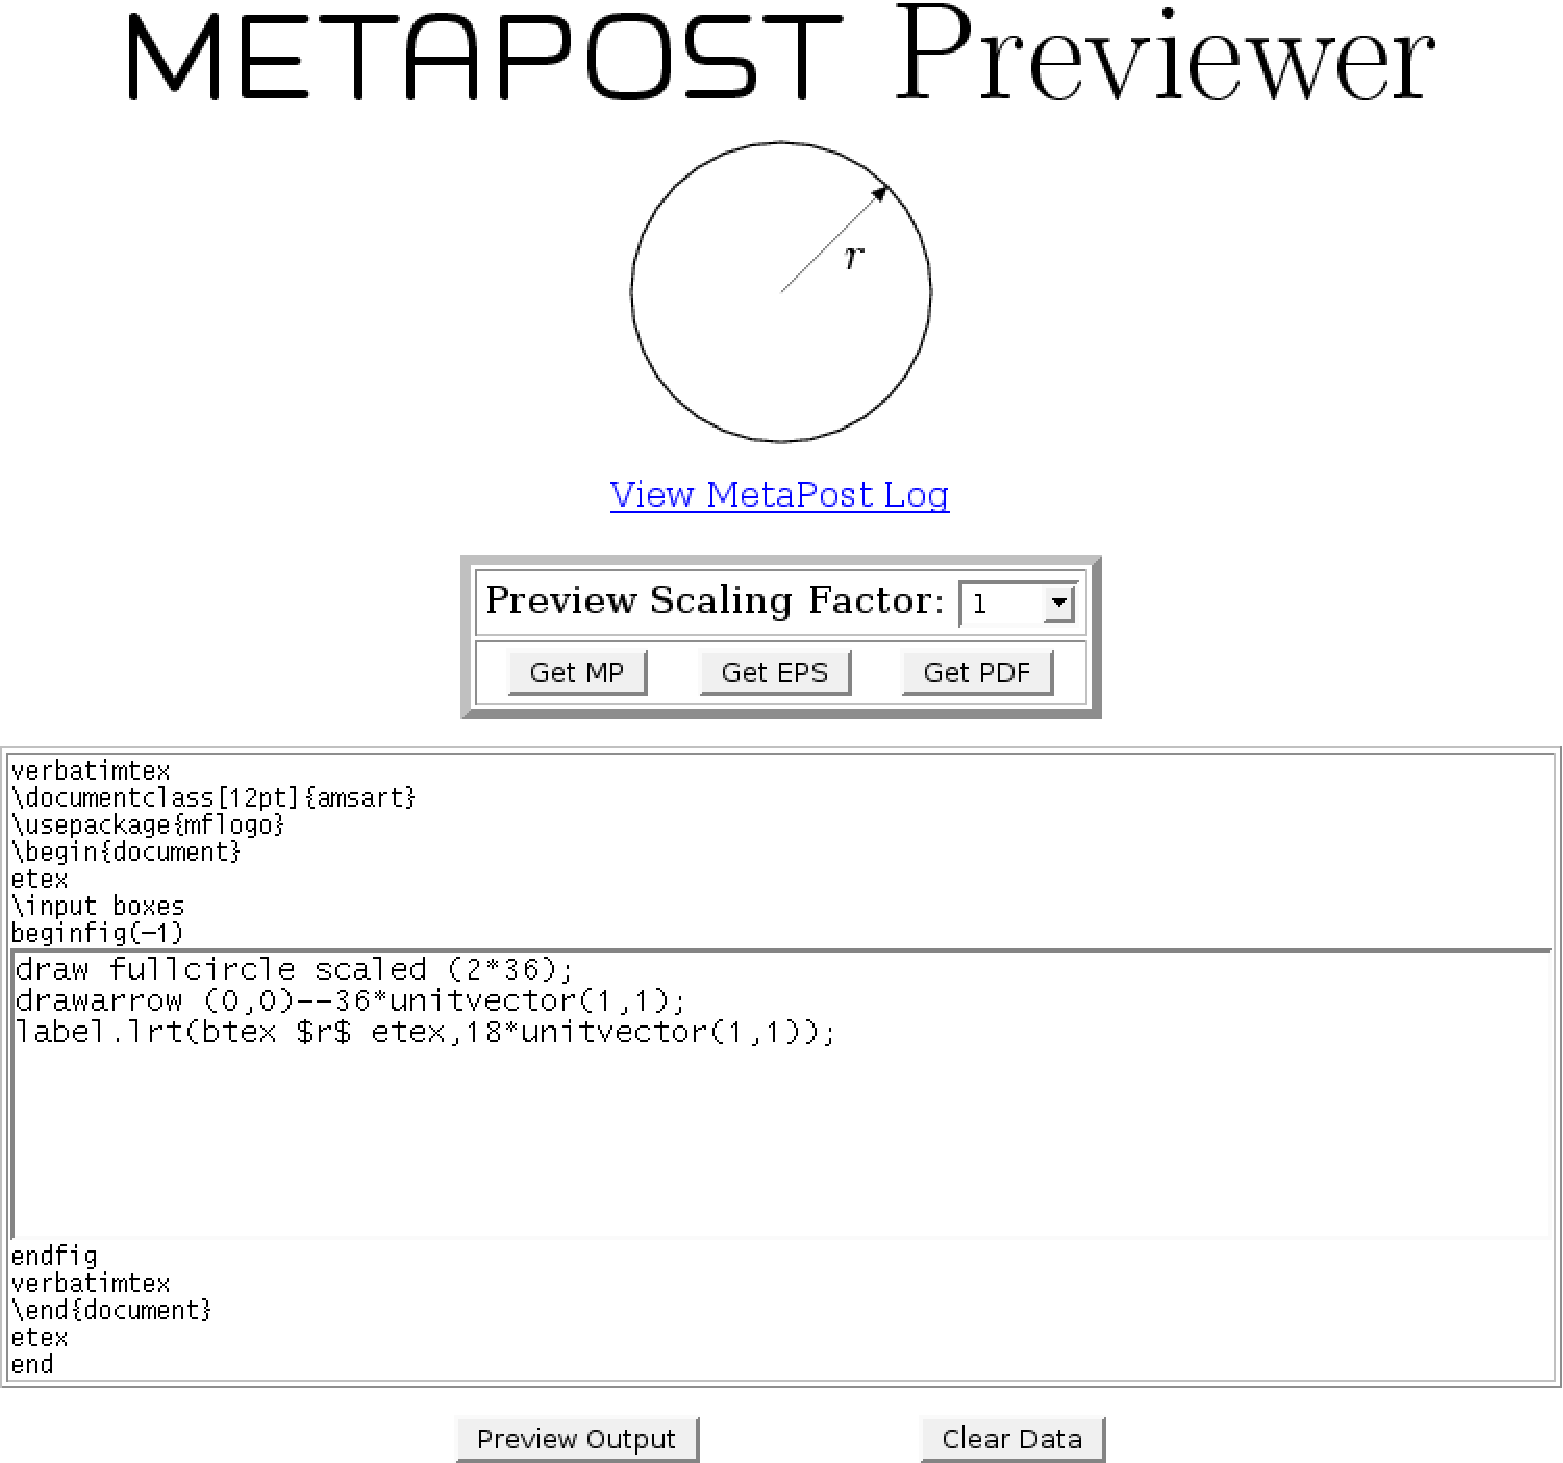
\includegraphics{previewer}}
		\caption{\MP{} Previewer}\label{fig:previewer}
	\end{center}
\end{figure*}

\begin{section}{\MP{} compilation}
A typical \MP{} source file consists of one or more figures.  Compilation of the source file generates an \EPS{} graphic for each figure.  These \EPS{} graphics are self-contained (i.e., the fonts used in labels are embedded into the graphic) provided that \lstinline{prologues:=3} is declared.

If \texttt{foo.mp} is a typical \MP{} source file with, then its contents are likely of the following form:
\begin{lstlisting}[xleftmargin=1.25\parindent]
prologues:=3;
beginfig(1);
   |\normalfont\textit{draw commands}|
endfig;
beginfig(2);
   |\normalfont\textit{draw commands}|
endfig;
|\dots|
beginfig(|\normalfont$n$|);
   |\normalfont\textit{draw commands}|
endfig;
end
\end{lstlisting}
Executing \begin{flushleft}\hspace*{1.25\parindent}\texttt{mpost foo.mp}\end{flushleft} yields the following output:
\begin{lstlisting}[xleftmargin=1.25\parindent]
This is MetaPost, Version |\normalfont$\langle$\textit{version}$\rangle$|
(foo.mp [1] [2] |\normalfont\ldots| [|\normalfont$n$|] )
|\normalfont$n$| output files written: foo.1 .. foo.|\rlap{\normalfont$n$}|
Transcript written on foo.log.
\end{lstlisting}

For users who just want to ``get started'' using \MP{}, a \MP{} previewer is available at \url{http://www.tlhiv.org/mppreview}.  This previewer (illustrated in Figure \ref{fig:previewer}) is simply a graphical interface to \MP{} itself.
It generates a single graphic with the option to save the output in \EPS{}, \PDF{}, and \SVG{} formats.  Users may also choose to save the source code and can view the compilation log to assist in debugging.
\end{section}
